\section{Phase 2: Define}

After conducting broad research on existing social robots, user needs, and contextual use within shared spaces like university buildings, we moved on to define more specific goals for our own robot. Our challenge was to design a friendly, autonomous assistant capable of organizing turns for a shared microwave, while maintaining a mobile and socially engaging presence.

In this phase, we started shaping our concept through rough prototypes to test:

\begin{itemize}
    \item Basic \textbf{movement mechanisms} using omnidirectional wheels.
    \item \textbf{Aesthetic identity}, considering a space between two separated bases for hiding the electronics.
    \item Key \textbf{functionalities}, for getting a proper movement of the robot.
\end{itemize}

The cardboard prototype that best adjusted to these ideas can be seen in the following picture.

\begin{figure}[H]
    \centering
    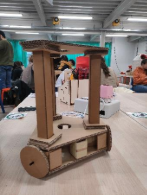
\includegraphics[width=0.5\linewidth]{../ReportMovementModule/images/Aspose.Words.728084da-df58-4b9d-a372-f65cffbdb23d.006.png}
    \caption{Cardboard prototype}
\end{figure}

These early tests helped us set a clearer direction for both technical and conceptual development, bridging the gap between idea and implementation.
